\documentclass[a4paper]{article}
\usepackage{fontspec}
\usepackage{fontenc}
\usepackage{extarrows}
\usepackage{chemfig}
\usepackage[version=4]{mhchem}
\usepackage{amsmath}
\usepackage{amssymb}
\usepackage{siunitx}
\usepackage{bigfoot}
\usepackage{fancyvrb}
\usepackage{tikz}
\usepackage{expl3}
\usepackage{calc}
\usepackage{geometry}
\geometry{left=2.5cm,right=2.5cm,top=2cm,bottom=3cm}
\usetikzlibrary{graphs, positioning, quotes, shapes.geometric}
\setmainfont{Hiragino Sans GB}

\title{元素化学笔记整理}
\author{胡译文}
\date{\today}

\makeatletter
\newcommand{\figcaption}{\def@captype{figure}\caption}
\newcommand{\tabcaption}{\def@captype{table}\caption}
\makeatother

\usepackage{hyperref}
\renewcommand\contentsname{目录}

\begin{document}
	\maketitle
	\renewcommand\contentsname{目录}
	\tableofcontents
	
	
	\newpage
	\section{\ce{Na}}
	\subsection{\ce{Na}单质}
	\subsubsection{物理性质}
	\begin{itemize}
		\item 银白色固体,有金属性光泽;
		\item 密度介于水和煤油之间,用煤油或石蜡保存;
		\item 熔点低;
		\item 质地较软,可以用小刀切割。
	\end{itemize}
	
	\subsubsection{化学性质}
		\paragraph{与非金属单质反应} 
			\begin{itemize}
				\item $\left\{\begin{array}{lr}
						\ce{4Na + O2 -> 2Na2O}\\
						\ce{2Na + O2 ->[\Delta] Na2O2}\\
					\end{array}\right.$
				\item $\ce{2Na + S -> Na2S}$
				\item $\ce{2Na + H2 ->[\Delta] 2NaH}$
				\item $\left\{\begin{array}{lr}
						\ce{2Na + Br2 -> 2NaBr}\\
						\ce{2Na + Cl2 ->[{点燃}] 2NaCl}\\
					\end{array}\right.$
			\end{itemize}
			\paragraph{与水反应}
			$\ce{2Na + 2H2O -> 2NaOH + H2 ^}$
			\begin{itemize}
				\item 浮:钠的密度比水小
				\item 溶:反应放热,钠的熔点低
				\item 游:生成氢气推动钠
				\item 响:反应剧烈
				\item 红:生成\ce{NaOH}遇到酚酞变红
			\end{itemize}
			\paragraph{与盐酸反应}
			$\ce{2Na + 2HCl -> 2NaCl + H2 ^}$
			\paragraph{与碱反应}
			实质是先与水反应,产物再和盐反应。
			\paragraph{与盐溶液反应}
			实质是先与水反应,产物再和盐反应(钠不能与盐溶液发生置换反应)。
			\begin{itemize}
				\item 钠与硫酸铜溶液
				$\left\{\begin{array}{lr}
					\ce{2Na + 2H20 -> 2NaOH + H2 ^}\\
					\ce{2NaOH + CuSO4 -> Na2SO4 + Cu(OH)2 v}\\
				\end{array}\right.$
			\end{itemize}
			\paragraph{与\ce{CO2}反应}
			$\left\{\begin{array}{lr}
				\ce{4Na + CO2 ->[\Delta] 2Na2O + C}\\
				\ce{4Na + 3CO2 ->[\Delta] 2Na2CO3 + C}\\
			\end{array}\right.$
		
	\subsubsection{钠的制取}
	$\left\{\begin{array}{lr}
		\ce{2NaCl(l) ->[{电解}] 2Na + Cl2 ^}\\
		\ce{2NaOH(l) ->[{电解}] 2Na + O2 ^ + H2 ^}\\
	\end{array}\right.$
	
	\subsubsection{钠的用途}
	\begin{itemize}
		\item 冶炼金属:$\ce{4Na + TiCl4(l) -> 4NaCl + Ti}$
		\item 原子反应导热剂
		\item 钠光灯
	\end{itemize}
	
	
	\subsection{\ce{Na}的化合物}
	
	\subsubsection{氧化钠和过氧化钠}
	\paragraph{比较氧化钠和过氧化钠}
	\renewcommand\arraystretch{2}
	\begin{center}
	\begin{tabular}{|c|c|c|}
		\hline
		名称&氧化钠&过氧化钠\\\hline
		化学式&\ce{Na2O}&\ce{Na2O2}\\\hline
		物理性质&白色固体&淡黄色固体\\\hline
		氧化物类型&碱性氧化物&过氧化物\\\hline
		制取&$\ce{4Na + O2 -> 2NaO}$&$\ce{2Na + O2 ->[\Delta] Na2O2}$\\\hline
		与水反应&$\ce{Na2O + H2O -> 2NaOH}$&$\ce{2Na2O2 + 2H2O -> 4NaOH + O2 ^}$\\\hline
		与酸反应&$\ce{Na2O + 2H+ -> 2Na+ + H2O}$&$\ce{2Na2O2 + 4H+ -> 4Na+ + 2H2O + O2 ^}$\\\hline
		与\ce{CO2}反应&$\ce{Na2O + CO2 -> Na2CO3}$&$\ce{2Na2O2 + 2CO2 -> 2Na2CO3 + O2}$\\\hline
		用途&制取烧碱&漂白剂、消毒剂、供氧剂\\\hline
	\end{tabular}
	\end{center}
	\paragraph{过氧化钠的强氧化性}
	\begin{itemize}
		\item 与\ce{SO2}反应:$\ce{Na2O2 + SO2 -> Na2SO4}$
		\item 投入\ce{FeCl2}溶液中生成\ce{Fe(OH)3}沉淀
		\item 投入氢硫酸,氧化硫化氢成硫单质,溶液浑浊
		\item 氧化\ce{SO3^2-}成\ce{SO4^2-}
		\item 使品红溶液褪色
	\end{itemize}
	
	\subsubsection{碳酸钠和碳酸氢钠}
	\paragraph{碳酸钠\ce{Na2CO3}}
	\begin{itemize}
		\item 俗名:纯碱、苏打
		\item 与盐酸反应:$\ce{Na2CO3 + 2HCl -> 2NaCl + H2O + CO2 ^}$
		\item 与\ce{Ca(OH)2}溶液反应:$\ce{Na2CO3 + Ca(OH)2 -> CaCO3 v + 2NaOH}$
		\item 与\ce{BaCl2}溶液反应:$\ce{Na2CO3 + BaCl2 -> BaCO3 v + 2NaCl}$
	\end{itemize}
	\paragraph{碳酸氢钠\ce{NaHCO3}}
	\begin{itemize}
		\item 俗名:小苏打
		\item 与盐酸反应:$\ce{NaHCO3 + HCl -> NaCl + H2O + CO2 ^}$
		\item 与过量\ce{Ca(OH)2}溶液反应:$\ce{Ca2+ + OH- + HCO3- -> CaCO3 v + H2O}$
		\item 与少量\ce{Ca(OH)2}溶液反应:$\ce{Ca2+ + 2OH- + 2HCO3- + Ca(OH)2 -> CaCO3 v + 2H2O + CO3^2-}$
		\item 与\ce{BaCl2}溶液反应:无明显现象
		\item 受热分解:$\ce{2NaHCO3 ->[\Delta] Na2CO3 + H2O + CO2 ^}$
	\end{itemize}
	\paragraph{相互转换}
	$\ce{Na2CO3 <=>[CO2 + H2O{或}H+][\Delta({固体}){或}OH-] NaHCO3}$
	\paragraph{鉴别\ce{Na2CO3}和\ce{NaHCO3}}
	\subparagraph{固体}
	根据热稳定性加热,能产生使澄清石灰水变浑浊的气体的是\ce{NaHCO3}
	\subparagraph{溶液}
	\begin{itemize}
		\item 与可溶性钙、钡盐生成沉淀的是\ce{Na2CO3}
		\item 与足量盐酸反应剧烈的是\ce{NaHCO3}
		\item 逐滴加盐酸先生成气体的是\ce{NaHCO3}
		\item 等物质的量pH值较大的是\ce{Na2CO3}
	\end{itemize}
	
	
	\newpage
	\section{Mg和Al}
	\subsection{Mg单质和Al单质}
	\subsubsection{化学性质}
	\paragraph{与非金属单质反应}
	\begin{itemize}
		\item 与\ce{O2}反应:$\left\{\begin{array}{lr}
					\ce{2Mg + O2 ->[{点燃}] 2MgO}(耀眼白光)\\
					\ce{4Al + 3O2 ->[{点燃}] 2Al2O3}\\
				\end{array}\right.$
		\item 与\ce{CO2}反应:$\ce{2Mg + CO2 ->[{点燃}] 2MgO + C}(耀眼白光,黑色固体生成)$
		\item 与\ce{N2}反应:$\ce{3Mg + N2 ->[{点燃}] Mg3N2}$
		\item 与卤素反应:$\left\{\begin{array}{lr}
					\ce{2Mg + Cl2 ->[{点燃}] 2MgCl2}\\
					\ce{2Al + 3Cl2 ->[{点燃}] 2AlCl3}\\
				\end{array}\right.$
		\item 与硫反应:$\left\{\begin{array}{lr}
					\ce{Mg + S ->[\Delta] MgS}\\
					\ce{2Al + 3S ->[\Delta] Al2S3}\\
				\end{array}\right.$
	\end{itemize}
	注意,镁在空气中燃烧时会同时发生前三个反应。
	\paragraph{与热水反应}
	$\left\{\begin{array}{lr}
		\ce{Mg + H2O({沸水}) -> Mg(OH)2 + H2 ^}\\
		\ce{2Al + 6H2O -> 2Al(OH)3 + 3H2 ^}\\
	\end{array}\right.$
	\paragraph{与酸发生置换反应}
	特例:铝在冷的浓硫酸或浓硝酸中钝化。
	\paragraph{铝热反应}
	可以与\ce{FeO}、\ce{Fe2O3}、\ce{Fe3O4}、\ce{Cr2O3}、\ce{MnO2}、\ce{V2O5}等氧化物反应。\\
	$\left\{\begin{array}{lr}
		\ce{2Al + Fe2O3 ->[{高温}] Al2O3 + 2Fe}\\
		\ce{2Al + Cr2O3 ->[{高温}] Al2O3 + 2Cr}\\
	\end{array}\right.$
	\\用途:焊接金属、冶炼难溶金属。
	\paragraph{与碱反应}
	镁不与碱反应。铝与强碱发生反应:$\ce{2Al + 2NaOH + 6H2 -> 2NaAlO2 + 4H2O + 3H2 ^}$
	\subsubsection{制备}
	\begin{itemize}
		\item 工业制铝:$\ce{2Al2O3(l) ->[{冰晶石}][{通电}] 4Al + 3O2 ^}$
		\item 工业制镁:$\left\{\begin{array}{lr}
						\ce{Mg2+ + 2OH- -> Mg(OH)2 v}\\
						\ce{Mg(OH)2 + 2HCl -> MgCl2 + H2O}\\
						\ce{MgCl2(l) ->[{通电}] Mg + Cl2 ^}\\
					\end{array}\right.$
	\end{itemize}
	
	
	\subsection{铝、氧化铝和氢氧化铝的两性}
	\paragraph{与酸反应}
	$\left\{\begin{array}{lr}
		\ce{2Al + 6H+ -> 2Al3+ + 3H2 ^}({非氧化性酸})\\
		\ce{Al2O3 + 6H+ -> 2Al3+ + 3H2O}\\
		\ce{Al(OH)3 + 3H+ -> Al3+ + 3H2O}\\
	\end{array}\right.$
	\paragraph{与强碱反应}
	$\left\{\begin{array}{lr}
		\ce{2Al + 2OH- + 2H2O -> 2AlO2- + 3H2 ^}\\
		\ce{Al2O3 + 2OH- -> 2AlO2- + H2O}\\
		\ce{Al(OH)3 + OH- -> AlO2- + 2H2O}\\
	\end{array}\right.$
	\paragraph{\ce{Al(OH)3}的电离}
	$\left\{\begin{array}{lr}
		\ce{Al(OH)3 <=> H+ + AlO2- + H2O}\\
		\ce{Al(OH)3 <=> Al3+ + OH-}\\
	\end{array}\right.$
	
	\subsection{铝离子和偏铝酸根}
	\subsubsection{铝离子}
	\paragraph{与\ce{NaOH}的相互滴加}
	缓慢滴加并搅拌
	\subparagraph{将\ce{NaOH}滴入\ce{Al3+}溶液中}
	\begin{enumerate}
		\item 先出现白色沉淀:$\ce{Al3+ + 3OH- -> Al(OH)3 v}\\$
		\item 后沉淀消失:$\ce{Al(OH)3 + OH- -> AlO2- + 2H2O}\\$
	\end{enumerate}
	\subparagraph{将\ce{Al3+}滴入\ce{NaOH}溶液中}
	\begin{enumerate}
		\item 先无明显现象:$\ce{Al3+ + 4OH- -> AlO2- + H2O}\\$
		\item 后产生白色沉淀:$\ce{Al3+ + 3AlO2- + 6H2O -> 4Al3(OH)3 v}\\$
	\end{enumerate}
	\paragraph{与氨水反应}
	$\ce{Al3+ + NH3*H2O -> Al(OH)3 v + 3NH4+}\\$
	\subsubsection{偏铝酸根}
	\paragraph{与强酸相互滴加}缓慢滴加并搅拌
	\subparagraph{将\ce{H2SO4}滴入\ce{AlO2-}溶液中}
	\begin{enumerate}
		\item 先出现白色沉淀:$\ce{AlO2- + H+ + H2O -> Al(OH)3 v}\\$
		\item 后沉淀消失:$\ce{Al(OH)3 + 3H+ -> Al3+ + 3H2O}\\$
	\end{enumerate}
	\subparagraph{将\ce{AlO2-}滴入\ce{H2SO4}溶液中}
	\begin{enumerate}
		\item 先无明显现象:$\ce{AlO2- + 4H+ -> Al3+ + 2H2O}\\$
		\item 后产生白色沉淀:$\ce{Al3+ + 3AlO2- + 6H2O -> 4Al3(OH)3 v}\\$
	\end{enumerate}
	\paragraph{与碳酸反应}
	立即生成\ce{Al(OH)3}沉淀且不溶解。
	\begin{itemize}
		\item \ce{CO2}过量:$\ce{AlO2- + 2H2O + CO2 -> Al(OH)3 v + HCO3-}\\$
		\item \ce{CO2}少量:$\ce{2AlO2- + 3H2O + CO2 -> 2Al(OH)3 v + CO3^2-}\\$
	\end{itemize}
	\paragraph{与铵盐溶液反应}
	$\ce{NH4+ + AlO2- + H2O -> Al(OH)3 v + NH3 ^}\\$
	
	\subsection{氢氧化铝}
	\subsubsection{制备}
	\begin{itemize}
		\item $\ce{Al3+ + NH3*H2O -> Al(OH)3 v + 3NH4+}\\$
		\item $\ce{AlO2- + 2H2O + CO2 -> Al(OH)3 v + HCO3-}\\$
		\item $\ce{Al3+ + 3AlO2- + 6H2O -> 4Al3(OH)3 v}\\$
	\end{itemize}
	
	\subsection{总结}
	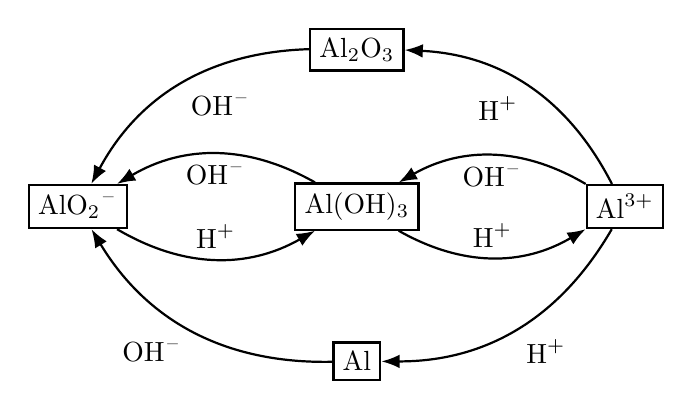
\begin{tikzpicture}[node distance=40pt, auto, thick]
		\node[draw] (Al2O3) {\ce{Al2O3}};
		\node[draw, below=of Al2O3] (AlOH) {\ce{Al(OH)3}};
		\node[draw, below=of AlOH] (Al) {\ce{Al}};
		\node[draw, right=60pt of AlOH] (Al3+) {\ce{Al^3+}};
		\node[draw, left=60pt of AlOH] (AlO2-) {\ce{AlO2-}};
		
		\draw[-Latex] (AlOH) [bend right] (AlO2-) edge node {\ce{H+}} (AlOH);
		\draw[-Latex] (AlO2-) [bend right] (AlOH) edge node {\ce{OH-}} (AlO2-);
		\draw[-Latex] (Al3+) [bend right] (AlOH) edge node {\ce{H+}} (Al3+);
		\draw[-Latex] (AlOH) [bend right] (Al3+) edge node {\ce{OH-}} (AlOH);
		\draw[-Latex] (Al2O3) [bend right] (Al3+) edge node {\ce{H+}} (Al2O3);
		\draw[-Latex] (AlO2-) [bend right] (Al2O3) edge node {\ce{OH-}} (AlO2-);
		\draw[-Latex] (Al) [bend left] (Al3+) edge node {\ce{H+}} (Al);
		\draw[-Latex] (AlO2-) [bend left] (Al) edge node {\ce{OH-}} (AlO2-);
	\end{tikzpicture}
	
	
	\newpage
	\section{Fe}
	\subsection{铁单质}
	\subsubsection{物理性质}
	\begin{itemize}
		\item 银白色固体,有金属性光泽;
		\item 容易被磁铁吸引;
		\item 地壳中居第四位;
	\end{itemize}
	
	\subsubsection{化学性质}
		铁元素性质活泼,有较强的还原性,主要化合价为+2价和+3价。
		\paragraph{与非金属单质反应} 
			\begin{itemize}
				\item $\ce{3Fe + 2O2 ->[{点燃}] Fe3O4}$
				\item $\ce{2Fe + 3Cl2 ->[{点燃}] FeCl3}$
				\item $\ce{Fe + S ->[\Delta] FeS}$
			\end{itemize}
		\paragraph{与水反应}
		铁在高温下与水蒸气反应
		$\ce{3Fe + 4H2O(g) ->[{高温}] Fe3O4 + 4H2}$
		\paragraph{与酸反应}
		铁遇到冷的浓硫酸或浓硝酸会钝化。
		\begin{itemize}
			\item 与非还原性酸:$\ce{Fe + 2H+ -> Fe^2+ + H2 ^}$
			\item 与还原性酸:$\ce{Fe + 4H+ + NO3- -> Fe^3+ + NO ^ + 2H2O}$
		\end{itemize}
		\paragraph{与盐溶液反应}
			\begin{itemize}
				\item 置换反应:$\ce{Fe + Cu^2+ -> Fe^2+ + Cu}$
				\item 与氯化铁溶液:$\ce{Fe + 2Fe^3+ -> 3Fe^2+}$ 
			\end{itemize}
			
	\subsection{铁的氧化物}
	\renewcommand\arraystretch{2}
	\begin{center}
	\begin{tabular}{|c|p{0.3\textwidth}<{\centering}|p{0.3\textwidth}<{\centering}|p{0.3\textwidth}<{\centering}|}
		\hline
		名称&氧化亚铁&氧化铁&四氧化三铁\\\hline
		俗称&-&铁红&磁性氧化铁\\\hline
		化学式&\ce{FeO}&\ce{Fe2O3}&\ce{Fe3O4}\\\hline
		化合价&+2&+3&+2、+3\\\hline
		物理性质&黑色粉末&红棕色粉末&黑色晶体\\\hline
		与\ce{CO}反应&$\ce{FeO + CO ->[\Delta] Fe + CO2}$&$\ce{Fe2O3 + 3CO ->[\Delta] 2Fe + 3CO2}$&$\ce{Fe3O4 + 4CO ->[\Delta] 3Fe + 4CO2}$\\\hline
		与\ce{H2}反应&$\ce{FeO + H2 ->[\Delta] Fe + H2O}$&$\ce{Fe2O3 + 3H2 ->[\Delta] 2Fe + 3H2O}$&$\ce{Fe3O4 + 4H2 ->[\Delta] 3Fe + 4H2O}$\\\hline
		与酸反应&$\ce{FeO + 2H+ -> Fe^2+ + H2O}$&$\ce{Fe2O3 + 6H+ -> 2Fe^3+ + 3H2O}$&$\ce{Fe3O4 + 8H+ -> Fe^2+ + 2Fe^3+ + 4H2O}$\\\hline
	\end{tabular}
	\end{center}

	\subsection{铁的水化物}
	\subsubsection{比较\ce{Fe(OH)2}和\ce{Fe(OH)3}}
	\begin{center}
	\begin{tabular}{|c|c|c|}
		\hline
		名称&氢氧化亚铁&氢氧化铁\\\hline
		化学式&\ce{Fe(OH)2}&\ce{Fe(OH)3}\\\hline
		物理性质&白色固体&红褐色固体\\\hline
		与酸反应&$\ce{Fe(OH)2 + 2H+ -> Fe^2+ + 2H2O}$&$\ce{Fe(OH)3 + 3H+ -> Fe^3+ + 3H2O}$\\\hline
		受热分解&$\ce{Fe(OH)2 ->[\Delta] FeO + H2O}$&$\ce{2Fe(OH)3 ->[\Delta] Fe2O3 + 3H2O}$\\\hline
		制备&$\ce{FeCl2 + 2NaOH -> Fe(OH)2 v + 2NaCl}$&$\ce{FeCl3 + 3NaOH -> Fe(OH)3 v + 3NaCl}$\\\hline
	\end{tabular}
	\end{center}
	\subsubsection{\ce{Fe(OH)2}和\ce{Fe(OH)3}的转化}
	\ce{Fe(OH)2}在空气中可以迅速被氧化成\ce{Fe(OH)3}。现象是由白色絮状沉淀迅速变成灰绿色,最后变成红褐色。
	反应方程式:\ce{4Fe(OH)2 + O2 + 2H2O -> 4Fe(OH)3}。
	
	\subsection{铁三角(铁、亚铁盐、铁盐)}
	\begin{tikzpicture}[node distance=40pt, auto, thick]
		\node[draw] (Fe) {\ce{Fe}};
		\node[below=104pt of Fe] (TEMP) {};
		\node[draw, right=60pt of TEMP] (Fe3+) {\ce{Fe^3+}};
		\node[draw, left=60pt of TEMP] (Fe2+) {\ce{Fe^2+}};
		
		\draw[-Latex] (Fe) (Fe3+) edge node {\ce{Cl2}} (Fe);
		\draw[-Latex] (Fe3+) [bend left] (Fe) edge node {\ce{Zn}} (Fe3+);
		\draw[-Latex] (Fe3+) (Fe2+) edge node {\ce{Fe}或\ce{Cu}} (Fe3+);
		\draw[-Latex] (Fe2+) [bend left] (Fe3+) edge node {\ce{HNO3}或\ce{Cl2}} (Fe2+);
		\draw[-Latex] (Fe2+) (Fe) edge node {\ce{Zn}} (Fe2+);
		\draw[-Latex] (Fe) [bend left] (Fe2+) edge node {\ce{Fe^3+}或\ce{H+}} (Fe);
	\end{tikzpicture}
	\paragraph{亚铁盐}
	含有\ce{Fe^2+}的溶液呈浅绿色,\ce{Fe^2+}既有氧化性,又有还原性。
	\paragraph{铁盐}
	含有\ce{Fe^3+}的溶液呈棕黄色, \ce{Fe^3+}具有氧化性。含有\ce{Fe^3+}的盐溶液遇到\ce{KSCN}溶液时变成红色。
	
	
	\newpage
	\section{Si}
	\subsection{硅单质}
	\subsubsection{物理性质}
	\begin{itemize}
		\item 分类:无定形硅、晶体硅(结构类似金刚石)
		\item 灰黑色晶状固体
		\item 质地较脆
		\item 半导体
	\end{itemize}
	\subsubsection{化学性质}
	\paragraph{与非金属单质反应} 
		\begin{itemize}
			\item $\ce{Si + O2 ->[{高温}] SiO2}$
			\item $\ce{Si + 2Cl2 ->[\Delta] SiCl4}$
			\item $\ce{Si + 2F2 -> SiF4}$
			\item $\ce{Si + C ->[{高温}] \underset{\text{金刚砂}}{SiC}}$
		\end{itemize}
	\paragraph{与水反应}
	$\underbrace{\ce{Si + H2O + 2NaOH -> Na2SiO3 + 2H2 ^}}_{\text{野外制氢}}$
		
	\subsection{硅的氧化物}
	\subsubsection{物理性质}
	\begin{itemize}
		\item 透明
		\item 硬度大
		\item 熔点高
	\end{itemize}
	\subsubsection{化学性质}
	\paragraph{酸性氧化物}
	\subparagraph{与强碱反应}
	$\underbrace{\ce{SiO2 + 2NaOH -> Na2SiO3 + H2O}}_{\text{装NaOH溶液不用玻璃塞}}$
	\subparagraph{与唯一一种酸氢氟酸反应}
	$\underbrace{\ce{SiO2 + 4Hf -> SiF2 ^ + 2 H2O}}_{\text{腐蚀玻璃、玻璃雕花}}$
	\subparagraph{与碱性氧化物反应}
	氧化硅与碱性氧化物反应,不与水反应(与水反应产物为硅酸,是沉淀,阻止反应进行)
	\begin{itemize}
		\item $\ce{SiO2 + Na2O ->[{高温}] Na2SiO3}$
		\item $\ce{SiO2 + CaO ->[{高温}] CaSiO3}$
	\end{itemize}
	\subparagraph{与碱性盐反应}
	\begin{itemize}
		\item $\underbrace{\ce{SiO2 + Na2CO3 ->[{高温}] Na2SiO3 + CO2 ^}}_{\text{制作玻璃}}$
		\item $\underbrace{\ce{SiO2 + CaCO3 ->[{高温}] CaSiO3 + CO2 ^}}_{\text{造渣反应}}$
	\end{itemize}
	\subparagraph{与碳反应}
	\begin{itemize}
		\item $\ce{SiO2 + 2C ->[{高温}] Si + 2CO ^}$
		\item $\ce{SiO2 + 3C ->[{高温}] SiC + 3CO ^}$
	\end{itemize}
	\subparagraph{精炼}
	\begin{enumerate}
		\item $\ce{SiO2 + 4Mg ->[{高温}] Mg2Si + 2MgO}$
		\item $\ce{Mg2Si + 4HCl -> 2MgCl2 + SiH4 ^}$
		\item $\ce{SiH4 + 2O2 -> SiO2 + 2H2O}$(自然)
	\end{enumerate}

	
	\subsection{硅的水化物(硅酸、原硅酸)}
	硅酸:\ce{H2SiO3}、、
	原硅酸:\ce{H4SiO4}
	\subsubsection{物理性质}
	白色胶状沉淀
	\subsubsection{化学性质}
	\paragraph{弱酸性}
	不使酸碱指示剂变色
	\subparagraph{硅酸电离}
	$\left\{\begin{array}{lr}
		\ce{H2SiO3 <=> H+ + HSiO3-}\\
		\ce{H2SiO3- <=> H+ + SiO3^2-}\\
	\end{array}\right.$
	\subparagraph{原硅酸电离}
	$\left\{\begin{array}{lr}
		\ce{H4SiO4 <=> H+ + H3SiO4-}\\
		\ce{H3SiO4- <=> H+ + H2SiO4^2-}\\
		\ce{H2SiO4- <=> H+ + HSiO4^3-}\\
		\ce{HSiO4- <=> H+ + SiO4^4-}\\
	\end{array}\right.$
	\paragraph{不稳定沉淀}
	\begin{itemize}
		\item $\ce{H4SiO4 -> H2SiO3 + H2}$
		\item $\ce{H2SiO3 ->[\Delta] SiO2 + H2O}$
		\item $\ce{H2SiO3 ->[\Delta] SiO2*xH2O + H2O}$
	\end{itemize}
	\paragraph{与强碱反应}
	\subparagraph{与氢氧化钠反应}
	$\ce{H2SiO3 + 2NaOH -> Na2SiO3 + 2H2O}$
	\subparagraph{不与氨气反应}
	$\ce{SiO3^2- + 2NH4+ -> H2SiO3 v + 2NH3 ^}$
	\paragraph{制备}
	
	\subsection{硅酸盐}
	\subsubsection{物理性质}
	\ce{K2SiO3}、\ce{Na2SiO3}溶于水,其余硅酸盐微溶于水。
	\subsubsection{化学性质}
	\begin{itemize}
		\item $\left\{\begin{array}{lr}
					\ce{Na2SiO3 + CO2 + H2O -> Na2CO3 + H2SiO3 v}\\
					\ce{Na2SiO3 + 2CO2 + 2H2O -> 2NaHCO3 + H2SiO3 v}\\
				\end{array}\right.$
		\item $\left\{\begin{array}{lr}
					\ce{Na2SiO3 + 6HF -> SiF4 ^ + 2NaF + 3H2O}\\
					\underbrace{\ce{CaSiO3 + 6HF -> SiF4 ^ + CaF2 + 3H2O}}_{\text{产物硅酸不稳定生成\ce{SiO2},继续与氢氟酸反应}}\\
				\end{array}\right.$
	\end{itemize}
	\subsubsection{硅酸盐的拆分}
	$活泼金属氧化物\longrightarrow 较活泼金属氧化物\longrightarrow 二氧化硅\longrightarrow 水$
	\begin{itemize}
		\item \ce{Na2SiO3}:\ce{Na2O*SiO2}
		\item \ce{CaSiO3}:\ce{CaO*SiO2}
		\item \ce{Al2(Si2O5)(OH)4)}:\ce{Al2O3*2SiO2*2H2O}
	\end{itemize}
	
	\subsection{用途与俗称}
	\subsubsection{用途}
	\begin{itemize}
		\item \ce{Si}(不透明):硅芯片、太阳能电池板
		\item \ce{SiO2}(透明):玻璃、石英玻璃、硅胶(\ce{mSiO2*nH2O},干燥剂)、光导纤维
		\item \ce{SiO3^2-}盐:水泥、陶瓷、防火材料等无机非金属材料
		\item \ce{H2SiO3}:制硅胶
	\end{itemize}
	\subsubsection{俗称}
	\begin{itemize}
		\item \ce{SiO2}:水晶、玛瑙、石英
		\item \ce{Na2SiO3}水溶液:水玻璃
		\item \ce{Na2SiO3}:泡花碱
	\end{itemize}
	
	
	\newpage
	\section{Cl}
	\paragraph{氯相关}
	\subparagraph{含氯酸}
	从上至下,酸性递增,氧化性递减。
	\begin{itemize}
		\item \ce{HClO}:次氯酸
		\item \ce{HClO2}:亚氯酸
		\item \ce{HClO3}:氯酸
		\item \ce{HClO4}:高氯酸
	\end{itemize}
	\subparagraph{卤素}
	\ce{F}、\ce{Cl}、\ce{Br}、\ce{I}
	\subparagraph{拟卤素}
	$\underset{\text{氰}}{\ce{CN}}$、$\underset{\text{硫氰}}{\ce{SCN}}$、$\underset{\text{氧氰}}{\ce{OCN}}$
	
	\subsection{盐酸}
	\subsubsection{物理性质}
	无色、有刺激性气味液体。
	\subsubsection{化学性质}
	\paragraph{酸性}
	产物中有盐
	\begin{itemize}
		\item $\ce{2H+ + Fe -> Fe^2+ + H2 ^}$
		\item $\ce{H+ + OH- -> H2O}$
		\item $\ce{2H+ + CaO -> Ca2+ + H2O}$
		\item $\ce{2H+ + CO3^2- -> CO2 ^ + H2O}$
	\end{itemize}
	\paragraph{氧化性}
	盐酸的氧化性由\ce{H+}体现
	\begin{itemize}
		\item $\ce{2H+ + Fe -> Fe^2+ + H2 ^}$
	\end{itemize}
	\paragraph{还原性}
	\begin{itemize}
		\item $\underbrace{\ce{4HCl({浓}) + MnO2 ->[\Delta] MnCl2 + CL2 ^ + 2H2O}}_{\text{实验室制氯气}}$
		\item $\left\{\begin{array}{lr}
				\ce{16HCl + 2KMnO4 -> 2KCl + 5Cl2 ^ + 2MnCl2 + 8H2O}\\
				\ce{14HCl + K2Cr2O7 -> 2KCl + 3Cl2 ^ + 2CrCl3 + 7H2O}\\
				\ce{6HCl + KClO3 -> KCl + 3Cl2 ^ + 3H2O}\\
				\ce{14HCl + PbO2 -> PbCl2 + Cl2 ^ + 2H2O}\\
				\ce{6HCl + NaBiO3 -> NaCl + Cl2 ^ + BiCl2 + 3H2O}\\
			\end{array}\right.$
	\end{itemize}
	\subsubsection{制备}
	\paragraph{工业}
	\begin{enumerate}
		\item $\ce{2NaCl + 2H2O ->[{高温}] 2NaOH + H2 ^ + Cl2 ^}$
		\item $\ce{H2 + Cl2 ->[{点燃}] 2HCl}$
	\end{enumerate}
	\paragraph{实验室}
	\begin{itemize}
		\item $\ce{NaCl + H2SO4({浓}) ->[\Delta] NaHSO4 + HCl ^}$
		\item $\ce{2NaCl + H2SO4({浓}) ->[\Delta] Na2SO4 + 2HCl ^}$
	\end{itemize}
	\subsection{氯气}
	\subsection{次氯酸}
	\subsection{含氯酸盐}
	
	
	\newpage
	\section{S}
	\subsection{硫化氢}
	\subsection{硫单质}
	\subsection{硫的氧化物}
	\subsection{亚硫酸}
	\subsection{硫酸}
	\subsection{含硫酸盐}
	
	
	\newpage
	\section{N}
	\subsection{氨气}
	\subsection{氮气}
	\subsection{氮的氧化物}
	\subsection{硝酸}
	\subsection{硝酸盐}
	
	
\end{document}
